\documentclass{article}%<<<1
\usepackage[margin=20mm]{geometry}
\usepackage{amsmath,amsfonts,mathrsfs}
\usepackage{unicode}
\usepackage{tikz}
\usetikzlibrary{trees,matrix}
% \usepackage{xypic}

\newtheorem{df}{Definition}
\newtheorem{prop}{Proposition}
\newtheorem{thm}{Theorem}
\DeclareMathOperator{\PGL}{PGL}
\DeclareMathOperator{\End}{End}
\DeclareMathOperator{\GL}{GL}
\DeclareMathOperator{\SL}{SL}
\def\scalar{\mathrm{scalar}}
\def\level#1{\mathrm{level}\pa{#1}}
\def\F{\mathbb{F}}
\def\mat#1{\begin{pmatrix}#1\end{pmatrix}}
\def\smat{\def\arraystretch{.6}\mat}
\let\limp\varprojlim
\def\acco#1{\left\{#1\right\}}
\def\pa#1{\left(#1\right)}
\def\abs#1{\left|#1\right|}
\def\card#1{\abs{#1}}
\def\XXX{\textbf{XXX}}
\def\labelitemi{--}
\let\ro\mathscr

\def\linkcounter#1#2{\edef\magic{\noexpand\let
  \expandafter\noexpand\csname c@#1\endcsname
  \expandafter\noexpand\csname c@#2\endcsname}\magic}

\begin{document}
The characteristic polynomial~$φ^2-4φ+43$ is split over~$ℚ_2$, with two
eigenvalues~$λ^{♯} ≡ 1 \pmod{4}$ and~$λ^{♭} ≡ -1 \pmod{4}$.
\section{The $ℓ$-adic Serre tree}%<<<1
\subsection{Definition}%<<<2
\begin{df}
The \emph{$ℓ$-adic Serre tree} of~$\GL_2$ is the set
$\PGL_2(ℚ_{ℓ})/\PGL_2(ℤ_{ℓ})$ (for the right-side action), equipped with
the distance
\begin{equation}
d(A, B) = v_{ℓ}(A^{-1} B) + v_{ℓ} (B^{-1} A)
\end{equation}
where $A$, $B$ are reduced (= with valuation~$0$) representatives of
their equivalence classes.
\end{df}

In other words, this is the space of lattices in~$ℚ_{ℓ}^2$, up to
homotheties, where two lattices~$Λ$ and~$Λ'$ are at a distance~$≤ n$ iff
there exist representatives~$L$ and~$L'$ such that
\begin{equation}
ℓ^n L ⊂ L' ⊂ L.
\end{equation}
The $ℓ$-adic Serre tree is regular with valence~$ℓ+1$.
Fix the standard lattice~$\mathrm{id}$ as the root of the tree. The
\emph{elementary lattices} are the~$ℓ+1$ lattices at distance~$1$
from the origin ; they are in bijection with~$ℙ^{1} \F_{ℓ}$, with
$ε_{∞} = \smat{1&0\\0&ℓ}$ and~$ε_i =
\smat{ℓ&i\\0&1}$ for~$i =0…ℓ-1$. Next figure shows the ball in the Serre
tree of~$\PGL_2(ℤ_{2})$ with radius~$3$ and centered on the standard
lattice.
\tikzstyle{level 1}=[sibling angle=120]
\tikzstyle{level 2}=[sibling angle=90]
\tikzstyle{level 3}=[sibling angle=70]
\begin{figure}[h] \begin{center}
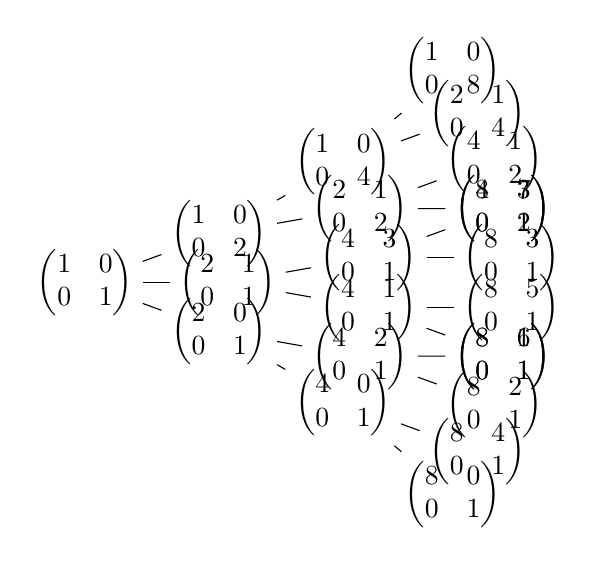
\begin{tikzpicture}[grow cyclic,level distance=12ex]%<<<
\node{$\mat{1&0\\0&1}$}
  child{ node{$\mat{2&0\\0&1}$}
    child { node {$\mat{4&0\\0&1}$}
      child { node {$\mat{8&0\\0&1}$} }
      child { node {$\mat{8&4\\0&1}$} }
    }
    child { node {$\mat{4&2\\0&1}$}
      child { node {$\mat{8&2\\0&1}$} }
      child { node {$\mat{8&6\\0&1}$} }
    }
  }
  child{ node{$\mat{2&1\\0&1}$}
    child { node {$\mat{4&1\\0&1}$}
      child { node {$\mat{8&1\\0&1}$} }
      child { node {$\mat{8&5\\0&1}$} }
    }
    child { node {$\mat{4&3\\0&1}$}
      child { node {$\mat{8&3\\0&1}$} }
      child { node {$\mat{8&7\\0&1}$} }
    }
  }
  child{ node{$\mat{1&0\\0&2}$}
    child { node {$\mat{2&1\\0&2}$}
      child { node {$\mat{4&3\\0&2}$} }
      child { node {$\mat{4&1\\0&2}$} }
    }
    child { node {$\mat{1&0\\0&4}$}
      child { node {$\mat{2&1\\0&4}$} }
      child { node {$\mat{1&0\\0&8}$} }
    }
  }
;
\end{tikzpicture}%>>>
\end{center} \end{figure}


Let~$α$ be a lattice at distance~$n$ from the origin. Then $α$~is
uniquely represented by its Hilbert normal form, which is a
matrix~$\smat{ℓ^{n-m}&b\\0&ℓ^m}$, where $m ≤ n$ and~$\min (m, n,
v_{ℓ}(b)) = 1$. The \emph{projective line} over a ring~$R$ is the set of
all vectors~$\smat{u\\v}$ of~$R^2$ such that~$u, v$ generate the unit
ideal of~$R$, modulo multiplication by invertible elements of~$R$.
We see that the kernel of~$α \pmod{ℓ^n}$ is generated by an element
of~$ℙ^1(ℤ/ℓ^nℤ)$. Moreover, this defines a canonical bijection
between~$ℙ^1(ℤ/ℓ^nℤ)$ and the set of points at distance~$n$; the image of
a point~$\smat{a\\1}$ is~$\smat{ℓ^n&a\\0&1}$, and the image of a
point~$\smat{1\\a}$, where~$m = v_{ℓ}(a) ≥ 1$, is~$\smat{ℓ^{n-m}&1\\0&a}$.

The \emph{ends} of the tree are the half-lines going to infinity from any
point; more formally, the topological space of ends is the projective
limit of the set of connected components of the tree deprived of a ball
of increasing radius. This set is isomorphic to~$ℙ^1(ℤ_{ℓ})$ as a
topological space with action of~$\PGL_2(ℤ_{ℓ})$.

\paragraph{Example: the 2-adic tree.}
The three elementary lattices are~$ε_{∞} =
\smat{1&0\\0&2}$, $ε_{0} = \smat{2&0\\0&1}$ and~$ε_{1} =
\smat{2&1\\0&1}$. Let~$g = \mat{0&1\\1&0} ∈ \PGL_2(ℤ_2)$. Then we see
that $g ε_{∞} = ε_0$, $g ε_0 = ε_{∞}$, and~$g ε_1 = \smat{0&1\\2&1} = ε_1
\smat{-1&0\\2&1}$, and is therefore equivalent to~$ε_1$ in the tree.
We check that the matrix~$g$ verifies~$g ε_i = ε_{1/i}$, where~$h: i ↦ 1/i$
is the homography with matrix~$\overline{g} = \smat{0&1\\1&0} ∈
\PGL_2(\F_2)$.

\subsection{Isogenies as points of the tree}%<<<2

Let~$k$ be a field of characteristic~$p ≠ ℓ$ and~$E/k$ be an elliptic
curve.

% A \emph{$ℓ^{∞}$-isogeny} is a class of equivalence of isogenies~$E
% → E'$ of order a power of~$ℓ$, modulo multiplication by a scalar on~$E$.
% (This is a path in the volcano). It is determined by its kernel~$Γ$,
% which is a $ℓ$-group of~$E$: a finite subgroup of~$E$, killed by a power
% of~$ℓ$, again defined modulo scalars.

The \emph{$ℓ$-adic Tate module}~$T_{ℓ}(E)$ and the associated vector
space~$V_{ℓ}(E)$ and $ℓ$-divisible group~$U_{ℓ}(E)$ are defined as
\begin{equation}
\begin{array}{rll}
T_{ℓ}(E) &= \limp E[ℓ^n]
  &= \acco {(x_n), x_0 = 0, ℓ · x_{n+1} = x_n};\\
V_{ℓ}(E) &= T_{ℓ}(E) ⊗_{ℤ_{ℓ}} ℚ_{ℓ}
  &= \acco {(x_n), ℓ^{∞} x_0 = 0, ℓ . x_{n+1} = x};\\
U_{ℓ}(E) &= V_{ℓ}(E) / T_{ℓ}(E)
  &= \acco {x_0 ∈ E, ℓ^{∞} x_0 = 0}.
\end{array}
\end{equation}
The $ℓ$-groups of~$E$ are the finite subgroups of~$U_{ℓ}(E)$. If $E$~is
ordinary then there exist isomorphisms
\begin{equation}
T_{ℓ}(E) ≃ ℤ_{ℓ}^2, \quad V_{ℓ}(E) ≃ ℚ_{ℓ}^2, \quad
  U_{ℓ}(E) ≃ (ℚ_{ℓ}/ℤ_{ℓ})^2.
\end{equation}

A \emph{$ℓ^n$-isogeny} is a class of equivalence of isogenies~$α: E → E'$
with cyclic kernel of order~$ℓ^n$, modulo elliptic curve isomorphisms. It
is determined by its action on the $ℓ$-adic Tate module~$T_{ℓ}(α)$, which
we again write~$α$; this is the matrix of a lattice in~$V_{ℓ}(E) ≃
V_{ℓ}(E')$, modulo scalars. This defines a natural bijection between the
set of $ℓ^n$-isogenies and the points of the Serre
tree~$\PGL_2(ℚ_{ℓ})/\PGL_2(ℤ_{ℓ})$ at a distance~$n$ from the origin.

% snake%<<<
% To an $ℓ$-group~$Γ ⊂ U_{ℓ}(E)$, one may associate the fibre product~$Λ(Γ) =
% V_{ℓ}(E) ×_{U_{ℓ}(E)} Γ$. In other words, this is the set of
% points~$(x_{n})$ of~$V_{ℓ}(E)$ such that~$x_0 ∈ Γ$. This is a lattice
% in~$V_{ℓ}(E)$, and multiplying~$Γ$ by a scalar multiplies~$Λ(Γ)$ by the
% same scalar; if~$\card{U} = ℓ^n$ then in the Serre tree, $d(1, Λ(Γ)) =
% n$. Moreover, this lattice fits in the exact sequence
% \begin{equation}
% 0 → T_{ℓ}(E) → Λ(Γ) → Γ → 0.
% \end{equation}
% This defines a bijection from the set of finite subgroups of~$U_{ℓ}(E)$
% (modulo scalars) to the Serre tree. Let~$E/Γ$ be the image of the isogeny
% with kernel~$Γ$; then the map~$T_{ℓ}(E) → T_{ℓ}(E/Γ)$ is the
% map~$T_{ℓ}(E) → Λ(Γ)$ above.

% Since finite subgroups
% correspond to isogenies, we may identify the following:
% 
% \begin{tabular}{ll}\toprule
% Vertices of the Serre tree & Distance from origin\\
% Matrices~$\smat{ℓ^m&a\\0&ℓ^n}$, $a ∈ [0,ℓ^m[$, $\min (m,n,v_{ℓ}(a)) = 0$
%   & $m+n$ \\
% Subgroups~$Γ$ of order~$ℓ^n$ & $n$ \\
% $ℓ^n$-isogenies & $n$ \\
% \bottomrule\end{tabular}
% 
% Let~$Γ$ be a finite subgroup and~$α: E → E^{Γ}$ be the corresponding
% isogeny. Since $V_{ℓ}$~is a $ℚ_{ℓ}$-vector spaces~$V_{ℓ}$, the
% map~$V_{ℓ}(α): V_{ℓ}(E) → V_{ℓ}(E^{Γ})$~is bijective, and we can deduce
% from the snake diagram
% \[\xymatrix {
%  & 0\ar@{=}[r]\ar[d] & 0\ar[r]\ar[d] & Γ\ar[d]
%  \ar`r[d]`[dd]+<0ex,5ex>`^d[ddlll]+<5ex,0ex>`d[dddll][dddll] \\
% 0\ar[r] & T_{ℓ}(E)\ar[r]\ar[d] & V_{ℓ}(E)\ar[r]\ar@{=}[d] &
%   U_{ℓ}(E)\ar[r]\ar[d] & 0\\
% 0\ar[r] & T_{ℓ}(E^{Γ})\ar[r]\ar[d] & V_{ℓ}(E^{Γ})\ar[r]\ar[d] &
%   U_{ℓ}(E^{Γ})\ar[r]\ar[d] & 0\\
%  & Γ \ar[r] & 0\ar@{=}[r] & 0
% }\]
% % \begin{tikzpicture}%<<< \matrix (m) [matrix of math nodes, row sep =
% % 2em, column sep = 3em] { & 0 & 0 & Γ & \\ 0 & T_{ℓ}(E) & V_{ℓ}(E) &
% % U_{ℓ}(E) & 0\\
% % 0 & T_{ℓ}(E^{Γ}) & V_{ℓ}(E^{Γ}) & U_{ℓ}(E^{Γ}) & 0\\ & Γ & 0 & 0\\};
% % \draw[=] (m-1-2)--(m-1-3); \draw[->] (m-1-3)--(m-1-4)--(m-4-2);
% % \draw[->] (m-2-1)--(m-2-2); \draw[->] (m-2-2)--(m-2-3); \draw[->]
% % (m-2-3)--(m-2-4); \draw[->] (m-2-4)--(m-2-5); \draw[->]
% % (m-3-1)--(m-3-2)--(m-3-3)--(m-3-4)--(m-3-5); \draw[->]
% % (m-1-2)--(m-2-2)--(m-3-2)--(m-4-2); \draw[->]
% % (m-1-4)--(m-2-4)--(m-3-4)--(m-4-4); \draw[->] (m-1-3)--(m-2-3);
% % \draw[=] (m-2-3)--(m-3-3); \draw[->] (m-3-3)--(m-4-3);
% % \end{tikzpicture}%>>>
% that~$0 → T_{ℓ}(E) → T_{ℓ} (E^{Γ}) → Γ → 0$~is exact, and that
% the $ℤ_{ℓ}$-modules $T_{ℓ}(E^{Γ})$ and~$Λ(Γ)$ are isomorphic as
% extensions of~$Γ$ by~$T_{ℓ}(E)$. Therefore, if $α$~is the matrix of~$Λ(Γ)
% ⊂ V_{ℓ}(E)$, then $α^{-1}$~is the matrix of~$T_{ℓ}(E) → T_{ℓ}(E^{Γ})$.
%>>>
\section{Action of the Frobenius endomorphism}%<<<1
\subsection{The isogeny volcano}%<<<2
All this was with coefficients in the algebraic closure. Now assume that
$E$~is defined over a finite field~$k = \F_q$, and let~$φ$ be the
Frobenius map on~$E$ and all associated $ℤ_{ℓ}$-modules $T_{ℓ}(E)$,
$V_{ℓ}(E)$ etc. Let~$φ = φ|T_{ℓ}(E)$. Then for any $ℓ^n$-isogeny~$α: E →
E^{α}$, we have~$φ^{α} = φ|T_{ℓ}(E^{α}) = α φ α^{-1}$.

\medskip

The Frobenius map is a root of the characteristic polynomial~$φ^2 - t φ +
q$. Let~$D = ℓ^{2r} d$ be the discriminant of~$φ$. The ring of integers
of~$ℚ_{ℓ}[φ]$ is generated by an element~$θ = √{d}$ if~$ℓ ≠ 2$, and~$θ =
(d+√{d})/2$ if~$ℓ = 2$. The orders of~$ℚ_{ℓ}[φ]$ are the rings~$\ro O_{n}
= ℤ_{ℓ}[ℓ^n θ]$. Fix~$r$ such that~$\ro O_{r} = ℤ_{ℓ}[φ]$. Then $\End E
⊗_{ℤ} ℤ_{ℓ}$ is isomorphic as a $ℤ_{ℓ}[φ]$-module to one of the $\ro
O_{n}[φ]$ for~$0 ≤ n ≤ r$. We call the integer~$n$ the \emph{level}
of~$E$ and write~$n = \level {E}$. We say that $E$~is \emph{maximal} if
its level is the maximal value~$r$. The action of Frobenius on~$T_{ℓ}(E)$
is given by the matrix~$(-t+ℓ^{n-\level{E}} θ)$. Therefore, the knowledge
of~$φ$ on~$T_{ℓ}(E)$ determines the level of~$E$: it is the greatest
integer~$r$ such that $φ$~is scalar (modulo~$r$).

The crater of the $ℓ$-volcano is non-trivial iff the characteristic
polynomial~$φ^2 -t φ + q$ splits over~$ℚ_{ℓ}$. In this case, the
horizontal isogenies are oriented by the eigenvalues~$λ_i$ of~$φ$:
namely, modulo~$ℓ^{n+1}$, the matrix of~$φ$ is diagonal with distinct
eigenvalues~$λ_1, λ_2$, so that the groups~$Γ_i = \ker (φ-λ_i) ∩
E[ℓ^{n+1}]$ are both cyclic and~$E[ℓ^{n+1}] = Γ_1 ⊕ Φ_2$. We say that the
$ℓ$-isogeny with kernel~$ℓ^{n} Γ_i$ is \emph{of type~$λ_i$}.

In this case, we may define the \emph{maximal}, or \emph{horizontal},
path~$Π$ on the Serre tree as the line connecting all maximal elliptic
curves in the $ℓ$-volcano. Let~$λ_1, λ_2$ be the two eigenvalues of~$φ$
over~$ℚ_{ℓ}$ and~$T_{ℓ}(E)_{λ_i}$ be the corresponding eigenspaces. Then
$Γ_i = T_{ℓ}(E)_{λ_i}/ℓ $ is a subgroup of order~$ℓ$, defining a
horizontal isogeny~$α_i: E → E/Γ_i$. The isogeny~$α_i$ is said to be
\emph{of type~$λ_i$}. This provides a canonical orientation on the
maximal path~$Π$, with one direction being of type~$λ_1$ and the other
being of type~$λ_2$. We write~$Π_1$ and~$Π_2$ for the corresponding ends
of~$Π$.

\subsection{Elementary step}%<<<2

Computing on elliptic curves enables the following ``elementary step''
operation: given an elliptic curve~$E$, a basis
of~$E[ℓ^{n+1}]$, the matrix of~$φ_{E} \pmod{ℓ^{n+1}}$ in this basis, and
an isogeny of degree~$ℓ$ $α: E → E'$, to compute $E'[ℓ^{n+1}]$ and the
matrix of~$φ_{E'} \pmod{ℓ^{n+1}}$.

Namely, let~$(P_1, P_2)$ be a basis of~$E[ℓ^{n+1}]$ and~$Φ$ be the matrix
of~$φ$ in this basis. We may choose~$P_1$ such that $ℓ^{n}
P_1$~generates~$α$. A basis of~$E'[ℓ^{n+1}]$ is~$(P'_1, P'_2)$ where
$P'_2 = α(P_2)$ and $P'_1$~is any point such that~$ℓP'_1 = α(P'_1)$.
Since the matrix of~$α: T_{ℓ}(E) → T_{ℓ}(E')$ is~$\smat{ℓ&0\\0&1}$, if
$φ = \smat{a&b\\c&d}$, then $φ' = α^{-1} φ α =
\smat{a&ℓ^{-1} b\\ℓc&d}$. Therefore, the knowledge of~$φ \pmod{ℓ^{n+1}}$
leaves only~$ℓ$ candidates for the value of~$ℓ^{-1} b$ and therefore
for~$φ' \pmod{ℓ^{n+1}}$.

\bigskip

We apply this to the case where $E$~is maximal and $n$~is its homothety
index, \emph{i.e.} the largest integer such that $φ_{E} \pmod{ℓ^{n}}$~is
scalar. Then knowledge of~$φ_{E} \pmod{ℓ^{n+1}}$ is enough to know
whether $φ_{E}$~splits in~$ℚ_{ℓ}$, and if it is the case, to determine
the orientation of the maximal path~$Π$.

By applying $d$~times the elementary step above, we may therefore
determine the point~$Π_{d}^{λ_i}$ of~$Π$ at a distance~$d$ in the
direction~$λ_i$.

\subsection{Computing an $ℓ'$-isogeny on the oriented path}%<<<2

A \emph{$ℓ'$-isogeny} between two curves~$E$ and~$E'$ is an isogeny~$ψ: E
→ E'$ of degree~$d$ prime to~$ℓ$. Thereafter, we assume that $E$, $E'$
are two rationally $ℓ'$-isogenous elliptic curves. This implies that the
map~$ψ: T_{ℓ}(E) → T_{ℓ}(E')$ is a $ℤ_{ℓ}[φ]$-isomorphism. In particular,
$E$~and~$E'$ have the same level.

\begin{prop}
Let~$Γ ⊂ U_{ℓ}(E)$ be represented by the lattice~$α$. Then $ψ(Γ) ⊂
U_{ℓ}(E')$ is represented by the lattice~$ψα$.
\end{prop}

From this we deduce that~$\level{(E')^{ψα}} = \level{E^{α}}$. If
$φ$~splits over~$ℚ_{ℓ}$, then $ψ$, as a map between the Serre tree of~$E$
and that of~$E'$, preserves the maximal paths~$Π$ and~$Π'$ and their
orientation by the eigenvalues of~$φ$.

\section{Example: curves over~$\F_{43}$ with 40 points}%<<<1

The volcano has a crater of $4$~curves $E_{j}$ where $j ∈ \acco { 12, 9,
29, 31}$ is the $j$-invariant. We know that $E_{12}$ and~$E_{29}$ are
5-isogenous.

$E_{12}: y^2 = x^3 + 30 x + 10$ has the 4-torsion points $P = (3, 16)$
and~$Q = (10, √{20})$, so that $φ ≡ \smat{1&\\&-1} \pmod{4}$. This proves
that the characteristic polynomial of~$φ$ splits over~$ℚ_{2}$, with two
eigenvalues~$λ^{♯} ≡ 1 \pmod{4}$ and $λ^{♭} ≡ -1 \pmod{4}$. Moreover
$2P = (34,0)$ and~$2Q = (19,0)$.

The 2-isogeny~$α_{12}^{♯} = ε_{0}$ with kernel~$2P$ is of type~$λ^{♯}$
and the Vélu formulas give
\[ α_{12}^{♯}: E_{12} → E_{9}, (x,y) → \pa{\frac{11x^2+13x+36}{x-34},
  27 y\frac{(x-22)(x-3)}{(x-34)^2}}, \]
where $E_9: y^2 = x^3+16x+25$. This curve has the 4-torsion points
$(10,14)$ and~$(1,√{-1})$. The basis of the $2$-torsion of~$E_{9}$
associated to~$α: E_{12} → E_{9}$ is $P' = α(P) = (36,0)$ and~$Q' = α(2Q)
= (26,0)$. Computing $4$-torsion, we see that only $P'+Q'$ is divisible
by 2, so that the next $♯$-isogeny is~$α_9 = ε_{1}$.

Therefore, we see that $α_{12}^{♯2} = ε_{1} ε_{0} = \smat{4&1\\0&1}$,
corresponding to the point~$∏^{♯} = \mat{1\\1} ∈ ℙ^1(ℤ/4ℤ)$.

Likewise, the $♭$-isogeny is~$α_{12}^{♭} = ε_{∞}$, with kernel
$2Q = (19,0)$:
\[ α_{12}^{♭}: E_{12} → E_{29}, (x,y) ↦ \pa{\frac{6x^2+15x+13}{x-19},
  y\frac{(x-28)(x-10)}{(x-19)^2}}, \]
where $E_{29}: y^2 = x^3 + 2x + 30$. The basis of $E_{29}[2]$ pushed
by~$α$ is~$α(2P) = (30,0)$ and~$α(Q) = (6,0)$. We see that~$α(2P)$ is
divisible while $α(Q)$~is divisible in~$\F_{43^2}$, so that the next
$♭$-isogeny is~$α_{29} = ε_{∞}$.

Therefore, $α_{12}^{♭2} = ε_{∞} ε_{∞} = \smat{1&0\\0&4}$, corresponding
to the point~$Π^{♭} = \smat{0\\1} ∈ ℙ^1(ℤ/4ℤ)$.

\medskip

Likewise we compute for~$E_{29}$: $P = (24,20)$, $2P = (30,0)$, $Q =
(20,√{29})$, $2Q = (6,0)$. Then $(2P) ≃ ε_{∞}$ generates the $♯$-isogeny
\[ α_{29}^{♯}: E_{29} → E_{12}, (x,y) ↦ \pa{\frac{(9x^2+31x+23)}{x-30},
  16y \frac{(x-24)(x-36)}{(x-30)^2}}. \]
We see that~$P' = α(P) = (33,0)$ and~$Q' = α(2Q) = (19,0)$. Therefore
$P'+Q'$ is divisible by~$2$, so that~$α_{12}^{♯} = ε_{1}$
and~$α_{29}^{♯2} = ε_{∞} ε_1 = \smat{2&1\\0&2} ≃ \smat{1\\2}$.

The $♭$-isogeny is generated by~$(2Q) = (6,0) ≃ ε_0$:
\[ α_{29}^{♯}: E_{29} → E_{31}, (x,y) ↦ \pa{\frac{(15x^2+39x+16)}{x-6},
   35y \frac{(x-20)(x-35)}{(x-6)^2}}. \]
We have~$P' = α(2P) = (35,0)$ and~$Q' = α(Q) = (37,0)$. Then $P'+Q'$
generates the next $♭$-isogeny and has matrix~$ε_1$. Therefore,
$α_{29}^{♭2} = ε_0 ε_1 = \smat{4&2\\0&1} ≃ \smat{2\\1}$.
% Likewise we compute for $E_{31}$: $P = (36,8)$, $2P = (35,0)$, $Q =
% (29,√{?})$, $2Q = (14,0)$. Then $(2P) = ε_{∞}$ generates the $♯$-isogeny
% \[ α_{31}^{♯}: E_{31} → E_{29}, (x,y) ↦ \pa{\frac{38x^2+3x+38}{x-35},
% 41y\frac{(x-34)(x-36)}{(x-35)^2}}. \]
% We see that~$P' = α(P) = (30,0)$ and~$Q' = α(2Q) = (6,0)$. Therefore,
% $P'$~is divisible by 2, so that~$α_{31}^{♯} = ε_{∞}$ and~$α_{31}^{♯2} =
% ε_{∞} ε_{∞} = \smat{1&0\\0&4} ≃ \smat{1\\0}$.
% 
% The $♭$-isogeny is generated by~$(2Q) = (14,0)$:
% \[ α_{31}^{♭}: E_{31} → E_{9}, (x,y) ↦ \pa{\frac{6x^2+2x+17}{x-14},
% y\frac{(x-42)(x-29)}{(x-14)^2}}. \]
% We have~$P' = α(2P) = (24,0)$ and~$Q' = α(Q) = (36,0)$. The next
% $♭$-isogeny is generated by~$P'+Q'$ and has matrix~$ε_1$.
% Therefore, we have $α_{31}^{♭2} = ε_{0} ε_{1} = \smat{4&2\\0&1} ≃
% \smat{2\\1}$.

\bigskip

From this we deduce that any $2'$-isogeny~$E_{12} → E_{29}$ is associated
to the homography of~$ℙ^1(ℤ/4ℤ)$ mapping~$\smat{1\\2}$ to~$\smat{1\\2}$
and $\smat{0\\1}$ to~$\smat{2\\1}$. It is therefore of the form
$\smat{u-4v&2v\\2(u-v)&v}$. Since it is invertible, we must have~$u,v = ±1$,
so that $ψ ≡ \smat{±1&2\\0&±1} \pmod{4}$. Both these
matrices commute to~$φ \pmod{4}$.

\bigskip

We can compute using the Vélu formula the 5-isogeny
\[ ψ: E_{12} → E_{29}, (x,y) ↦ \pa{\frac{10x^5+12x^4+35x^3+28x^2+37x+8}
  {(x-1)^2(x-7)^2}, 21y \frac{x(x-14)(x-17)(x-20)(x-23)(x-36)}
  {(x-1)^3(x-7)^3}}. \]


\end{document}
